\part{Module introduction}
\frame{\partpage}

\begin{frame}{Module Outline}
	\begin{itemize}
		\item Enhance the student’s creative practice by developing a series of playable prototypes
		\item This will be accomplished by:
		\begin{itemize}
			\item Developing a series of Game Prototypes
			\item These will be based on a prompt given out in class
			\item We by essence doing a bunch of Game Jams in the module
			\item Allows you to develop your own Design process and voice
		\end{itemize}
	\end{itemize}
\end{frame}


\begin{frame}{Assignment}
	\begin{itemize}
		\item \textbf{Assignment 1: Portfolio of Game Prototypes - 100\%}
			\begin{itemize}
				\item The aim of the assignment is to develop your 'voice' as a designer
				\item Create \textbf{4} prototypes during the course of the module
				\item Create a 10 min Postmortem video at the end of each prototype
				\item Select \textbf{3} prototypes for the final submission
				\item Create a final 10 min video which sums up your learning as a Designer
			\end{itemize}
	\end{itemize}
\end{frame}

\begin{frame}{Assignment}
	\begin{itemize}
		\item See LearningSpace for assignment brief
		\item See MyFalmouth for deadlines
	\end{itemize}
\end{frame}

\begin{frame}{Assignment Tips}
	\begin{itemize}
		\item Ideation is key, don't just jump into the idea
		\item Use the full 2 weeks to complete the prototype
		\item Don't be afraid to fail, fail fast and often
		\item Kill you darlings, if a prototype isn't working move onto another one
		\item Pick up a new tool or skill during the module
	\end{itemize}
\end{frame}

\begin{frame}{Module Roadmap}
	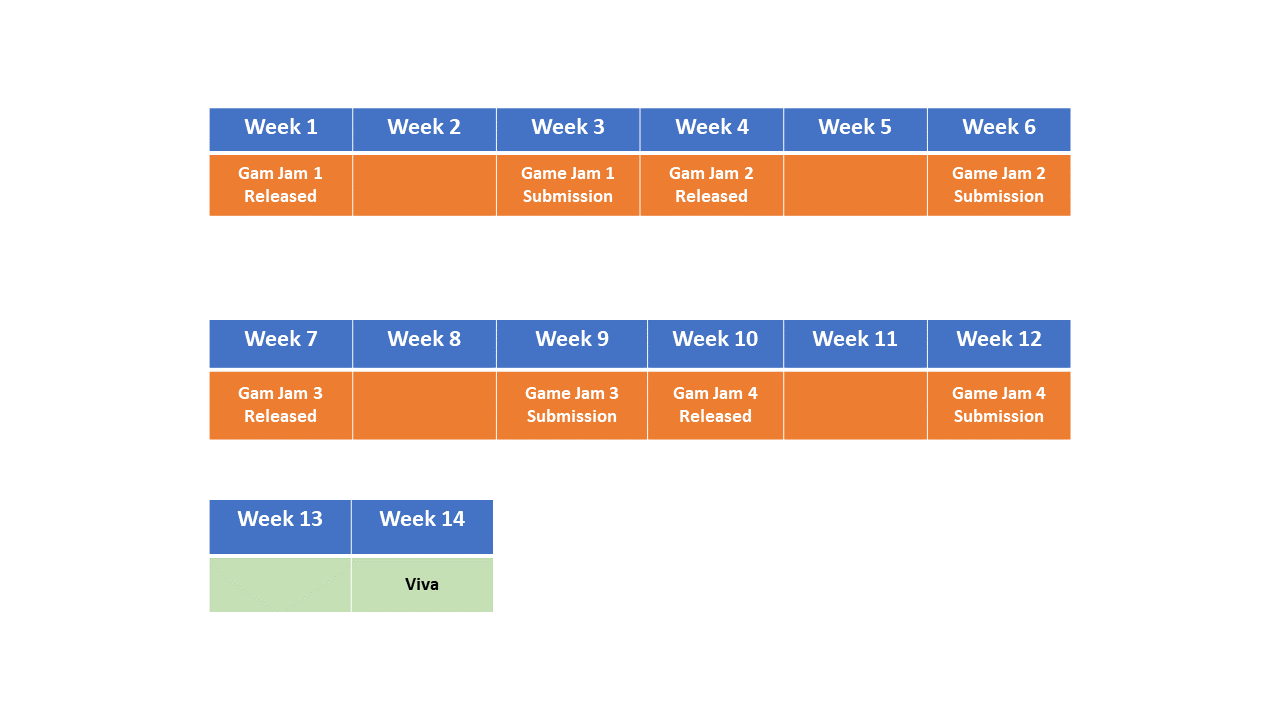
\includegraphics[width=1.0\textwidth]{GAM702_Road_Map}
\end{frame}